%%%%%%%%%%%%%%%%%%%%%%%%%%%%%%%%%%%%%%%%%
% Lachaise Assignment
% LaTeX Template
% Version 1.0 (26/6/2018)
%
% This template originates from:
% http://www.LaTeXTemplates.com
%
% Authors:
% Marion Lachaise & François Févotte
% Vel (vel@LaTeXTemplates.com)
%
% License:
% CC BY-NC-SA 3.0 (http://creativecommons.org/licenses/by-nc-sa/3.0/)
% 
%%%%%%%%%%%%%%%%%%%%%%%%%%%%%%%%%%%%%%%%%

%----------------------------------------------------------------------------------------
%	PACKAGES AND OTHER DOCUMENT CONFIGURATIONS
%----------------------------------------------------------------------------------------

\documentclass{article}

%%%%%%%%%%%%%%%%%%%%%%%%%%%%%%%%%%%%%%%%%
% Lachaise Assignment
% Structure Specification File
% Version 1.0 (26/6/2018)
%
% This template originates from:
% http://www.LaTeXTemplates.com
%
% Authors:
% Marion Lachaise & François Févotte
% Vel (vel@LaTeXTemplates.com)
%
% License:
% CC BY-NC-SA 3.0 (http://creativecommons.org/licenses/by-nc-sa/3.0/)
% 
%%%%%%%%%%%%%%%%%%%%%%%%%%%%%%%%%%%%%%%%%

%----------------------------------------------------------------------------------------
%	PACKAGES AND OTHER DOCUMENT CONFIGURATIONS
%----------------------------------------------------------------------------------------

\usepackage{dirtree}
\usepackage{float} % here for H placement parameter
\usepackage{amsmath,amsfonts,stmaryrd,amssymb} % Math packages
\usepackage[dvipsnames]{xcolor}
\usepackage{enumerate} % Custom item numbers for enumerations
\usepackage{hyperref}
%\usepackage[ruled,vlined]{algorithm2e} % Algorithms
\usepackage{algpseudocode}
\usepackage{algorithm}
\usepackage[framemethod=tikz]{mdframed} % Allows defining custom boxed/framed environments

\usepackage{listings} % Required for insertion of code

\newcommand{\randomcolor}{%
  \definecolor{randomcolor}{RGB}
   {
    \pdfuniformdeviate 256,
    \pdfuniformdeviate 256,
    \pdfuniformdeviate 256
   }%
  \color{randomcolor}%
}

\definecolor{codegreen}{rgb}{0,0.6,0}
\definecolor{codegray}{rgb}{0.5,0.5,0.5}
\definecolor{codepurple}{rgb}{0.58,0,0.82}
\definecolor{backcolour}{rgb}{1,1,1}
\lstdefinestyle{mystyle}{
    backgroundcolor=\color{backcolour},   
    commentstyle=\color{codegreen},
    keywordstyle=\color{magenta},
    numberstyle=\tiny\color{codegray},
    stringstyle=\color{codepurple},
    basicstyle=\ttfamily\footnotesize,
    breakatwhitespace=false,         
    breaklines=true,                 
    captionpos=b,                    
    keepspaces=true,                 
    numbers=left,                    
    numbersep=5pt,                  
    showspaces=false,                
    showstringspaces=false,
    showtabs=false,                  
    tabsize=2
}
\renewcommand{\lstlistingname}{Código}% Listing -> Algorithm
\lstset{style=mystyle}


%\usepackage{listings} % File listings, with syntax highlighting
%\lstset{
%	basicstyle=\ttfamily, % Typeset listings in monospace font
%}

%----------------------------------------------------------------------------------------
%	DOCUMENT MARGINS
%----------------------------------------------------------------------------------------

\usepackage{geometry} % Required for adjusting page dimensions and margins

\geometry{
	paper=a4paper, % Paper size, change to letterpaper for US letter size
	top=2.5cm, % Top margin
	bottom=3cm, % Bottom margin
	left=2.5cm, % Left margin
	right=2.5cm, % Right margin
	headheight=14pt, % Header height
	footskip=1.5cm, % Space from the bottom margin to the baseline of the footer
	headsep=1.2cm, % Space from the top margin to the baseline of the header
	%showframe, % Uncomment to show how the type block is set on the page
}

%----------------------------------------------------------------------------------------
%	FONTS
%----------------------------------------------------------------------------------------

\usepackage[utf8]{inputenc} % Required for inputting international characters
\usepackage[T1]{fontenc} % Output font encoding for international characters

\usepackage{XCharter} % Use the XCharter fonts

%----------------------------------------------------------------------------------------
%	COMMAND LINE ENVIRONMENT
%----------------------------------------------------------------------------------------

% Usage:
% \begin{commandline}
%	\begin{verbatim}
%		$ ls
%		
%		Applications	Desktop	...
%	\end{verbatim}
% \end{commandline}

\mdfdefinestyle{commandline}{
	leftmargin=10pt,
	rightmargin=10pt,
	innerleftmargin=15pt,
	middlelinecolor=black!50!white,
	middlelinewidth=2pt,
	frametitlerule=false,
	backgroundcolor=black!5!white,
	frametitle={Command Line},
	frametitlefont={\normalfont\sffamily\color{white}\hspace{-1em}},
	frametitlebackgroundcolor=black!50!white,
	nobreak,
}

% Define a custom environment for command-line snapshots
\newenvironment{commandline}{
	\medskip
	\begin{mdframed}[style=commandline]
}{
	\end{mdframed}
	\medskip
}

%----------------------------------------------------------------------------------------
%	FILE CONTENTS ENVIRONMENT
%----------------------------------------------------------------------------------------

% Usage:
% \begin{file}[optional filename, defaults to "File"]
%	File contents, for example, with a listings environment
% \end{file}

\mdfdefinestyle{file}{
	innertopmargin=1.6\baselineskip,
	innerbottommargin=0.8\baselineskip,
	topline=false, bottomline=false,
	leftline=false, rightline=false,
	leftmargin=2cm,
	rightmargin=2cm,
	singleextra={%
		\draw[fill=black!10!white](P)++(0,-1.2em)rectangle(P-|O);
		\node[anchor=north west]
		at(P-|O){\ttfamily\mdfilename};
		%
		\def\l{3em}
		\draw(O-|P)++(-\l,0)--++(\l,\l)--(P)--(P-|O)--(O)--cycle;
		\draw(O-|P)++(-\l,0)--++(0,\l)--++(\l,0);
	},
	nobreak,
}

% Define a custom environment for file contents
\newenvironment{file}[1][File]{ % Set the default filename to "File"
	\medskip
	\newcommand{\mdfilename}{#1}
	\begin{mdframed}[style=file]
}{
	\end{mdframed}
	\medskip
}

%----------------------------------------------------------------------------------------
%	NUMBERED QUESTIONS ENVIRONMENT
%----------------------------------------------------------------------------------------

% Usage:
% \begin{question}[optional title]
%	Question contents
% \end{question}

\mdfdefinestyle{question}{
	innertopmargin=1.2\baselineskip,
	innerbottommargin=0.8\baselineskip,
	roundcorner=5pt,
	nobreak,
	singleextra={%
		\draw(P-|O)node[xshift=1em,anchor=west,fill=white,draw,rounded corners=5pt]{%
		Pregunta \theQuestion\questionTitle};
	},
}

\newcounter{Question} % Stores the current question number that gets iterated with each new question

% Define a custom environment for numbered questions
\newenvironment{question}[1][\unskip]{
	\bigskip
	\stepcounter{Question}
	\newcommand{\questionTitle}{~#1}
	\begin{mdframed}[style=question]
}{
	\end{mdframed}
	\medskip
}

%----------------------------------------------------------------------------------------
%	WARNING TEXT ENVIRONMENT
%----------------------------------------------------------------------------------------

% Usage:
% \begin{warn}[optional title, defaults to "Warning:"]
%	Contents
% \end{warn}

\mdfdefinestyle{warning}{
	topline=false, bottomline=false,
	leftline=false, rightline=false,
	nobreak,
	singleextra={%
		\draw(P-|O)++(-0.5em,0)node(tmp1){};
		\draw(P-|O)++(0.5em,0)node(tmp2){};
		\fill[black,rotate around={45:(P-|O)}](tmp1)rectangle(tmp2);
		\node at(P-|O){\color{white}\scriptsize\bf !};
		\draw[very thick](P-|O)++(0,-1em)--(O);%--(O-|P);
	}
}

% Define a custom environment for warning text
\newenvironment{warn}[1][Warning:]{ % Set the default warning to "Warning:"
	\medskip
	\begin{mdframed}[style=warning]
		\noindent{\textbf{#1}}
}{
	\end{mdframed}
}

%----------------------------------------------------------------------------------------
%	INFORMATION ENVIRONMENT
%----------------------------------------------------------------------------------------

% Usage:
% \begin{info}[optional title, defaults to "Info:"]
% 	contents
% 	\end{info}

\mdfdefinestyle{info}{%
	topline=false, bottomline=false,
	leftline=false, rightline=false,
	nobreak,
	singleextra={%
		\fill[black](P-|O)circle[radius=0.4em];
		\node at(P-|O){\color{white}\scriptsize\bf i};
		\draw[very thick](P-|O)++(0,-0.8em)--(O);%--(O-|P);
	}
}

% Define a custom environment for information
\newenvironment{info}[1][Info:]{ % Set the default title to "Info:"
	\medskip
	\begin{mdframed}[style=info]
		\noindent{\textbf{#1}}
}{
	\end{mdframed}
}
 % Include the file specifying the document structure and custom commands

%----------------------------------------------------------------------------------------
%	ASSIGNMENT INFORMATION
%----------------------------------------------------------------------------------------

\title{IC-2023: Proyecto} % Title of the assignment

\author{Luis Ballado\\ \texttt{luis.ballado@cinvestav.mx}} % Author name and email address

\date{CINVESTAV UNIDAD TAMAULIPAS --- \today} % University, school and/or department name(s) and a date

%----------------------------------------------------------------------------------------
\algnewcommand\algorithmicforeach{\textbf{for each}}
\algdef{S}[FOR]{ForEach}[1]{\algorithmicforeach\ #1\ \algorithmicdo}

\begin{document}

\maketitle % Print the title

%----------------------------------------------------------------------------------------
%	INTRODUCTION
%----------------------------------------------------------------------------------------

\section{Instrucciones para ejecución}

\begin{info} % Information block
  Se adjunta la liga al repositorio, donde se encuentran los códigos\\
  \href{https://github.com/luisballado/InteligenciaComputacional/tree/master/proyecto}{ver código en github}\\
\end{info}

\begin{info} % Information block
  Se hacen uso de las siguientes bibliotecas de Python
  \begin{itemize}
  \item argparse - creación de banderas para alimentar el programa
  \item \href{https://pypi.org/project/fuzzylogic/}{fuzzylogic}  - construcción de Lógica Borrosa
  \item \href{https://pypi.org/project/traci/}{traci} - Interfaz de SUMO en su versión de python
  \item \href{https://pypi.org/project/tabulate/}{tabulate} - generación de tablas en línea de comandos
  \item \href{https://pypi.org/project/sumolib/}{sumolib} - Bibliotecas SUMO
  \end{itemize}
\end{info}

\begin{enumerate} 

\item \href{https://sumo.dlr.de/docs/Downloads.php}{Instalar Simulador SUMO} en una distro LINUX

  \begin{commandline}
    \begin{verbatim}
      $ sudo add-apt-repository ppa:sumo/stable
      $ sudo apt-get update
      $ sudo apt-get install sumo sumo-tools sumo-doc
    \end{verbatim}
 \end{commandline}
  
\item Instalar dependencias con el archivo requirements.txt incluido en los archivos. (python >= 3)
  \begin{commandline}
 \begin{verbatim}
  $ pip install -r requirements.txt
  \end{verbatim}
 \end{commandline}
  
\item Clonar el repositorio
  
\begin{commandline}
 \begin{verbatim}
  $ git clone https://github.com/luisballado/InteligenciaComputacional.git
  $ cd InteligenciaComputacional
  $ cd proyecto
  $ cd fuzzy_semaphore
 \end{verbatim}
\end{commandline}

\newpage
\item Descripción Archivos \\

  Dentro del repositorio se sigue la siguiente estructura para organizar los archivos del proyecto (archivos xml que definen los parámetros del mapa a construir en el simulador SUMO):\\
  
  \dirtree{%
    .1 fuzzy\_semaphore/.
    .2 logica\_borrosa.py.
    .2 requirements.txt.
    .2 sumo\_run.py.
    .2 victoria\_cluster.add.xml.
    .2 victoria\_cluster.net.xml.
    .2 victoria\_cluster.net.xml.gz.
    .2 victoria\_cluster.neteditcfg.
    .2 victoria\_cluster.rou.xml.
    .2 victoria\_cluster.sumocfg.
    .2 victoria\_cluster\_ligero.rou.xml.
    .2 victoria\_cluster\_medio.rou.xml.
    .2 victoria\_cluster\_pesado.rou.xml.
  }

\end{enumerate} 

\begin{itemize}
\item \textbf{logica\_borrosa.py} - Clase Lógica Borrosa donde se hacen los cálculos
\item \textbf{sumo\_run.py} - Programa principal para ejecutar el simulador con el mapa de CD. Victoria.
\item \textbf{victoria\_cluster.\*} - Archivos generados por el Wizard al construir el mapa seleccionado
\end{itemize}

%---------------------------------------------------------------------

\newpage
\section{Valores de los Parámetros}

En la ejecución del programa se incluyen banderas para su ejecución con Interfaz gráfica o no, y también la cantidad de trafico a generar.

\begin{itemize}
\item --show True ó --show False
\item --traffic Bajo ó --traffic Medio ó --traffic Alto
\end{itemize}

Dependiendo de la versión de python en su máquina se correria de la siguiente forma:

\begin{commandline}
 \begin{verbatim}
  $ python3 sumo_run.py --show True --traffic Bajo
 \end{verbatim}
\end{commandline}

\subsection{Lógica Difusa}

Se propone un control de lógica difusa para el control de los semaforos, partiendo de la premisa que podemos contar la cantidad de carros gracias al sensor lane area detector, así también contabilizar el tiempo de su última participación en el cluster.\\

\subsubsection{Dominio}
\begin{itemize}
\item Trafico : [0 - 100]
\item Tiempo  : [0 - 240]
\item Tiempo Semaforo : [0 - 60]
\end{itemize}
\subsubsection{Conjuntos}
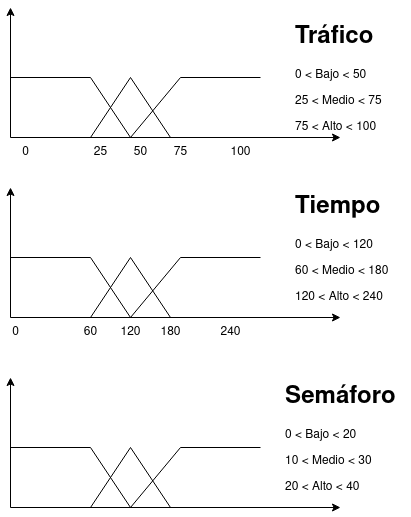
\includegraphics[scale=0.6]{logica_difusa.png}

%---------------------------------------------------------------------

\newpage
\section{Estadísticas}


%---------------------------------------------------------------------
\section{Referencias}

\href{https://sumo.dlr.de/docs/Simulation/Traffic_Lights.html}{Traffic Lights Control}\\
\href{https://pypi.org/project/traci/}{Interfaz SUMO-Python}\\
\href{https://github.com/ethanpng2021/sumo-example/blob/main/2021-05-01-22-25-37/sumo_run.py}{Ejemplo Manejo Interfaz Python-SUMO}\\
\href{https://sumo.dlr.de/docs/TraCI/Lane_Area_Detector_Value_Retrieval.html}{Lane Area Detector}\\
\href{https://cst.fee.unicamp.br/sites/default/files/sumo/sumo-roadmap.pdf}{Tutorial SUMO - A Road Map SUMO}
\end{document}

